\documentclass[border=2pt]{standalone}

%% Fonts
%\usepackage{fontspec}
%% Default Features
%\defaultfontfeatures{
%	Mapping=tex-text,
%	Ligatures=TeX,
%}
%% Serif Font
%\setmainfont[
%	UprightFont=EBGaramond-Regular,
%	ItalicFont=EBGaramond-Italic,
%	BoldFont=EBGaramond-Bold,
%	BoldItalicFont=EBGaramond-BoldItalic,
%]{EB Garamond}
%% Mono Font
%\setmonofont[
%	UprightFont=JetBrainsMonoNL-Regular,
%	ItalicFont=JetBrainsMonoNL-Italic,
%	BoldFont=JetBrainsMonoNL-Bold,
%	BoldItalicFont=JetBrainsMonoNL-BoldItalic,
%]
%{JetBrains Mono}

% Tikz
\usepackage{tikz}
\usetikzlibrary{calc, positioning, shapes}

% Colors
%\definecolor{myyellow}{RGB}{255, 255, 191}
%\definecolor{mygreen}{RGB}{171, 221, 164}
%\definecolor{myblue}{RGB}{216, 225, 246}
% Dimensions
\def\deltadim{0.2pt}
\def\innersep{3pt}
\def\servershift{1.5cm}
\def\shortenlen{2pt}
% Pipeline stages
\def\stageslinewidth{1.5pt}
\def\stagesdrawcolor{magenta!100}
\def\stagesfillcolor{magenta!20}
\def\stagesheight{30pt}
\def\stageswidth{66pt}
%% Followers
\def\followersnum{4}
% Connections
\def\connectionshift{0.35}
\def\labelinnersep{1.5pt}

% Styles
\tikzset{
	% labels
	label/.style={
		font=\large\ttfamily,
		align=center,
	},
	% Pipeline stages
	stages/.style={
		shape=rectangle,
		draw=\stagesdrawcolor,
		line width=\stageslinewidth,
		fill=\stagesfillcolor,
		rounded corners=0cm,
		minimum height=\stagesheight,
		minimum width=\stageswidth,
		label,
		inner ysep=0pt,
		inner xsep=\innersep,
		outer sep=0pt,
	},
	% connections
	connection/.style={
		very thick,
		-stealth,
		shorten <=\shortenlen , shorten >=\shortenlen
	}
}

\begin{document}
	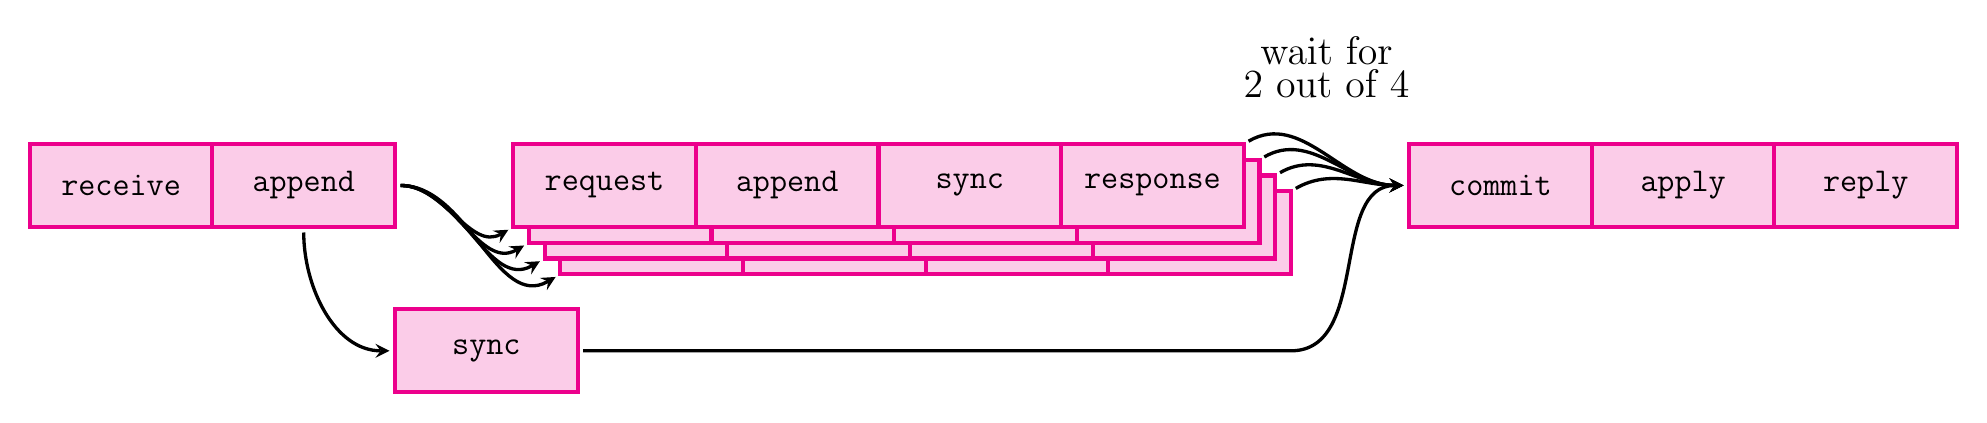
\begin{tikzpicture}
		% Leader replicates log
		\node[
			stages
		] (leader_receive) {receive};
		%
		\node[
			stages,
			anchor=west,
		] (leader_append) at (leader_receive.east) {append};
		%
		\pgfmathsetmacro{\displacement}{(\followersnum-1) * \deltadim}
		\node[
			stages,
			anchor=west,
			yshift=-\servershift
		] (leader_sync) at 
		  ($(leader_append.east) + (0,-\displacement)$) {sync};
		
		% Followers receive AppendEntries
		\foreach \i in {\followersnum,...,1} {
			\pgfmathsetmacro{\displacement}{(\i-1) * \deltadim}
			\node[
				stages,
				anchor=west,
				shift={(\servershift,0)},
			] (follower_request\i) at 
			  ($(leader_append.east) + (\displacement,-\displacement)$) 
			  {request};
			%
			\node[
				stages,
				anchor=west,
			] (follower_append\i) at (follower_request\i.east) {append};
			%
			\node[
				stages,
				anchor=west,
			] (follower_sync\i) at (follower_append\i.east) {sync};		
			%
			\node[
				stages,
				anchor=west,
			] (follower_response\i) at (follower_sync\i.east) {response};		
		}
		
		% Leader applies committed entries
		\node[
			stages,
			anchor=west,
			shift={(\servershift,0)},
		] (leader_commit) at 
		  (follower_response1.east-|follower_response\followersnum.east) 
		  {commit};
		%
		\node[
			stages,
			anchor=west,
		] (leader_apply) at (leader_commit.east) {apply};
		%
		\node[
			stages,
			anchor=west,
		] (leader_reply) at (leader_apply.east) {reply};
		
		% Connections
		%% Leader -> sync
		\draw [
			connection
		] (leader_append.south) to [out=270, in=180] (leader_sync.west);
		%% Leader -> Followers
		\foreach \i in {\followersnum,...,1} {
			\draw [
				connection
			] (leader_append.east) to[out=0, in=210] (follower_request\i.south west);
		}
		%% Followers -> Leader
		\foreach \i in {\followersnum,...,1} {
			\draw [
				connection
			] (follower_response\i.north east) to[out=30, in=180] (leader_commit.west);
		}
		%% sync -> Leader
		\draw [
			connection
		] (leader_sync.east) -- 
		  (follower_response\followersnum.east|-leader_sync) to[out=0, in=180]
		  (leader_commit.west);
		
		% Labels
		\pgfmathsetmacro{\consensus}{int(\followersnum/2)}
		\node [
			align=center,
			shift={(0,1.5)}
		]
			at ($(follower_response1)!0.5!(leader_commit)$) 
			{\Large wait for \\\Large\consensus\ out of \followersnum};
	\end{tikzpicture}
\end{document}